\section{Experiments}\label{sec:experiments}
With an objective to improve designers' productivity in developing FPGA accelerators, the key goal
of QuickDough is to reduce compilation and development time for such hardware-software system.
However, to warrant the merit of such framework, the performance and implementation overhead of the
generated acceleration system should remain competitive to ones that are developed with conventional
manual design efforts. For that purpose, we have conducted a series of experiments on end-to-end
application performance, compilation time, and implementation overhead of QuickDough. In each case,
multiple configurations of the overlay were experimented in order to study their area-performance
tradeoffs. The results are then compared against a typical manual accelerator design methodology
that employs conventional vendor-provided high-level synthesis tools. Finally, we studied the
scalability of the proposed overlay design and investigated how such regular design may benefit
large accelerator designs in the future.


%In order to evaluate QuickDough, we had a benchmark implemented on Zedboard \cite{zedboard} using
%both QuickDough and Vivado HLS and then performed a comprehensive comparison of the two different
%sets of implementations on performance, compilation time, implementation overhead and scalability. 

The experiment section is organized as follows. We will first briefly introduce the benchmark
programs in the following subsection and explain the basic experiment setup in
\secref{subsec:setup}. Then we will elaborate the comparison of performance, compilation,
implementation overhead and scalability in \secref{subsec:performance}-\secref{subsec:scalability}
respectively. 

\subsection{Benchmark} \label{subsec:benchmark}
Four applications were used as benchmark in this work, namely, matrix-matrix multiplication (MM), a
finite impulse response (FIR) filter, a K-mean clustering algorithm (KM) and a Sobel edge detector
(SE). For each application, three input with small (S), medium (M) and large (L) datasets were used,
forming a total of 12 combinations. The basic parameters and configurations of the benchmark are
illustrated in \tabref{tab:benchmark-config} and the loop structures of the programs are shown in
\tabref{tab:loop-structure}. 

\begin{table}
  \tbl{Detailed Configurations of the Benchmark \label{tab:benchmark-config}}{
  \centering
  \resizebox{0.8\columnwidth}{!}{
  \begin{tabular}{l|l|l|l|l}
  \hline
  Benchmark & MM & FIR & SE & KM \\ \hline
  Parameters & Matrix Size & \tabincell{l}{\# of Input/\\ \# of Taps+1} & \tabincell{l}{ \# of Vertical Pixels/\\ \# of Horizontal Pixels} & \tabincell{l}{\# of Nodes/Centroids/\\Dimension} \\ \hline
  S & 10 & 40/50 & 8/8 & 20/4/2 \\ \hline
  M & 100 & 10000/50 & 128/128 & 5000/4/2  \\ \hline
  L & 1000 & 100000/50 & 1024/1024 & 50000/4/2 \\ \hline
  \end{tabular}
  }
  }
\end{table}


\subsection{Experiment Setup} \label{subsec:setup}
The Xilinx implementation tools were run on a computer with Intel Core i5-3230M CPU and
\SI{8}{\giga\byte} of RAM. The resulting hardware-software platform was targeted at the Zedboard with
an XC7Z020 FPGA. Software components of the user applications ran on the embedded ARM processor,
while the hardware accelerators were implemented in the programmable logic.

To develop accelerators with QuickDough, the SCGRA overlay was first developed in ISE 14.7 and was
subsequently imported as an IP core in XPS 14.7. With the IP core, the SCGRA overlay based FPGA
accelerator was further integrated and implemented in PlanAhead 14.7.

As a comparison, we also developed accelerators following a typical implementation flow.
In particular, Vivado HLS 2013.3 was used to transform the compute kernels into hardware IP Catalogs.
They were then integrated into the rest of the FPGA acceleration system using Vivado 2013.3.

Furthermore, 2 accelerator configurations were employed in each design methodology. In the case of
building custom accelerators with Vivado HLS, 2 systems, called HS and HL in the
results, which included a \SI{2}{\kilo\byte} and \SI{64}{\kilo\byte} I/O buffer respectively were
used. In the case of QuickDough, the 2 systems, labeled as QS and QL were developed,
which included a $2\times 2$ and $5 \times 5$ processing arrays respectively. The basic
configurations of the QS and QL are listed in \tabref{tab:scgra-config}.

\begin{table}
\footnotesize 
\tbl{SCGRA Configuration \label{tab:scgra-config}}{
\centering
  \resizebox{0.9\columnwidth}{!}{
\begin{tabular}{c|c|c|c|c|c}

\hline
{SCGRA Topology} & {SCGRA Size} & {Instruction Mem} & {Data Memory} & {I/O Data Buffer} & {Addr Buffer} \\ \hline
{Torus} & {$2 \times 2$, $5 \times 5$} & {$1024 \times 72$ bits} & {$256 \times 32$ bits} & {$2048 \times 32$ bits} & {$4096 \times 18$ bits} \\ \hline
\end{tabular}
}
}
\end{table}

\subsubsection{Loop unrolling and grouping}
In our benchmark, multi-level loops form the compute intensive sections that are accelerated by FPGAs.
The structure for these loops are shown in \tabref{tab:loop-structure}.

\begin{table}
\footnotesize 
  \tbl{Complete Loop Structure of the Benchmark \label{tab:loop-structure}}{
  \centering
  \resizebox{0.75\columnwidth}{!}{
  \begin{tabular}{l|l|l|l|l}
  \hline
  Benchmark & MM & FIR & SE & KM \\ \hline
  S & $10 \times 10 \times 10$ & $40 \times 50$ & $8 \times 8 \times 3 \times 3$ & $20 \times 4 \times 2$ \\ \hline
  M & $100 \times 100 \times 100$ & $10000 \times 50$ & $128 \times 128 \times 3 \times 3$ & $5000 \times 4 \times 2$  \\ \hline
  L & $1000 \times 1000 \times 1000$ & $100000 \times 50$ & $1024 \times 1024 \times 3 \times 3$ & $50000 \times 4 \times 2$ \\ \hline
  \end{tabular}
  }
  }
\end{table}

To increase the amount of concurrent compute operations available, these loops were first unrolled
by a factor of $U$. Input and output data for $G$ invocations of the unrolled loop body are
subsequently grouped into individual transfers to amortize the cost for communication between
hardware and software. As explained, the unrolling factor $U$ and grouping factor $G$ have
significant impact on the overall application performance for both QuickDough and for any typical
HLS design methodology.

\tabref{tab:loop-unrolling-setup-vivado} shows the loop unrolling and grouping arrangement for
generating accelerators using typical high-level synthesis tools in this work. In these cases, while
larger loop unrolling factors typically result in better simulated performance, additional
hardware resource must usually be consumed. The increased resource usage may lead to a lowered
implementation frequency on the FPGA and thus lower overall performance. At the same time, larger
group size is beneficial to data reuse and helps to amortize the initial communication cost.
However, additional on-chip memory resources must be utilized as I/O buffer instead of being spent
on computation, potentially limiting the performance of the hardware accelerator. In this work, we
set the loop unrolling factor just large enough to reach the best simulated performance.
Furthermore, we also set grouping factor to large enough to fully utilize the on-chip buffer in the
2 accelerator configurations. 

\begin{table}
\footnotesize
\centering
\tbl{Loop Unrolling \& Grouping Setup Of Accelerators Using Direct HLS Based Design Framework \label{tab:loop-unrolling-setup-vivado}}{
  \resizebox{0.8\columnwidth}{!}{
\begin{tabular}{ll|l|l|l|l}
\hline
\multicolumn{2}{l|}{\multirow{2}{*}{Application}} & \multicolumn{2}{l|}{HL} & \multicolumn{2}{l}{HS} \\ \cline{3-6}
\multicolumn{2}{l|}{} & Unrolling Factor & Group Structure & Unrolling Factor & Group Structure \\ \hline

\multicolumn{1}{l|}{\multirow{3}{*}{MM}} & S & $2 \times 10 \times 10$ & $10 \times 10 \times 10$ & $2 \times 10 \times 10$ & $10 \times 10 \times 10$  \\ \cline{2-6} 
\multicolumn{1}{l|}{}                    & M & $1 \times 1 \times 100$ & $100 \times 100 \times 100$ & $1 \times 100$ & $10 \times 100$  \\ \cline{2-6} 
\multicolumn{1}{l|}{}                    & L & $1 \times 500$ & $50 \times 1000$ & 500 & 1000  \\ \hline

\multicolumn{1}{l|}{\multirow{3}{*}{FIR}} & S & $2 \times 50$ & $40 \times 50$ & $2 \times 50$ & $40 \times 50$  \\ \cline{2-6} 
\multicolumn{1}{l|}{} & M & $2 \times 50$ & $10000 \times 50$ & $2 \times 50$ & $1000 \times 50$  \\ \cline{2-6} 
\multicolumn{1}{l|}{} & L & $2 \times 50$ & $50000 \times 50$ & $2 \times 50$ & $1000 \times 50$  \\ \hline

\multicolumn{1}{l|}{\multirow{3}{*}{SE}} & S & $1 \times 2 \times 3 \times 3$ & $8 \times 8 \times 3 \times 3$ & $1 \times 2 \times 3 \times 3$ & $8 \times 8 \times 3 \times 3$ \\ \cline{2-6} 
\multicolumn{1}{l|}{} & M & $1 \times 1 \times 3 \times 3$ & $128 \times 128 \times 3 \times 3$ & $1 \times 1 \times 3 \times 3$ & $23 \times 128 \times 3 \times 3$ \\ \cline{2-6} 
\multicolumn{1}{l|}{} & L & $1 \times 1 \times 3 \times 3$ & $75 \times 1024 \times 3 \times 3$ & $1 \times 1 \times 3 \times 3$ & $4 \times 1024 \times 3 \times 3$ \\ \hline

\multicolumn{1}{l|}{\multirow{3}{*}{KM}} & S & $20 \times 4 \times 2$ & $20 \times 4 \times 2$ & $20 \times 4 \times 2$ & $20 \times 4 \times 2$  \\ \cline{2-6} 
\multicolumn{1}{l|}{} & M & $5 \times 4 \times 2$ & $5000 \times 4 \times 2$ & $5 \times 4 \times 2$ & $1000 \times 4 \times 2$  \\ \cline{2-6} 
\multicolumn{1}{l|}{} & L & $5 \times 4 \times 2$ & $25000 \times 4 \times 2$ & $5 \times 4 \times 2$ & $1000 \times 4 \times 2$  \\ \hline
\end{tabular}
}
}
\end{table}


Similar loop unrolling and grouping sizes were chosen carefully for the experiments targeting the
QuickDough overlay as shown in  \tabref{tab:loop-unrolling-setup-scgra}. In the case of the
QuickDough overlay, a large unrolling factor leads to a larger input DFG, which affects the SCGRA
array size, instruction ROM size, as well as data memory size. The group size has direct impact on
I/O buffer size, address buffer size, and communication latency. In this work, we manually adopted
the unrolling factor and group size to the two SCGRA configurations to balance computation and
communication.


\begin{table}
\footnotesize 
\centering
\tbl{Loop Unrolling and Grouping Setup For Accelerators Using QuickDough \label{tab:loop-unrolling-setup-scgra}}{
  \resizebox{0.7\columnwidth}{!}{
\begin{tabular}{l|l|l|l|l|l}
\hline
\multicolumn{2}{l|}{\multirow{2}{*}{Application}} & \multicolumn{2}{l|}{QS} & \multicolumn{2}{l}{QL}
\\ \cline{3-6}
\multicolumn{2}{l|}{} & \tabincell{l}{Unrolling \\ Factor} &
\tabincell{l}{Group \\ Structure} & \tabincell{l}{Unrolling \\ Factor} & \tabincell{l}{Group \\ Structure} \\ \hline

\multirow{3}{*}{MM} & S & $10 \times 10 \times 10$ & $10 \times 10 \times 10$ & $10 \times 10 \times
10$  & $10 \times 10 \times 10$  \\ \cline{2-6} 
            & M & $5 \times 100$  & $10 \times 100$ & $5 \times 100$  & $10 \times 100$  \\
\cline{2-6} 
            & L & 200 & 1000 & 200 & 1000  \\ \hline

\multirow{3}{*}{FIR} & S & $40 \times 50$  & $40 \times 50$ & $40 \times 50$  & $40 \times 50$  \\
\cline{2-6} 
                  & M & $20 \times 50$ & $100 \times 50$ & $50 \times 50$  & $250 \times 50$ \\
\cline{2-6} 
                  & L & $20 \times 50$ & $100 \times 50$ & $50 \times 50$ & $250 \times 50$ \\ \hline

\multirow{3}{*}{SE} & S & $4 \times 8 \times 3 \times 3$ & $8 \times 8 \times 3 \times 3$ & $8
\times 8 \times 3 \times 3$ & $8 \times 8 \times 3 \times 3$   \\ \cline{2-6} 
                  & M & $4 \times 8 \times 3 \times 3$ & $8 \times 8 \times 3 \times 3$ & $23 \times
8 \times 3 \times 3$ & $65 \times 8 \times 3 \times 3$  \\ \cline{2-6} 
                  & L & $4 \times 4 \times 3 \times 3$ & $16 \times 4 \times 3 \times 3$ & $16 \times 4 \times 3 \times 3$ & $16 \times 4 \times 3 \times 3$  \\ \hline

\multirow{3}{*}{KM} & S & $20 \times 4 \times 2$ & $20 \times 4 \times 2$ & $20 \times 4
\times 2$ & $20 \times 4 \times 2$  \\ \cline{2-6} 
                 & M & $25 \times 4 \times 2$ & $125 \times 4 \times 2$ & $125 \times 4 \times 2$ &
$500 \times 4 \times 2$  \\ \cline{2-6} 
                 & L & $25 \times 4 \times 2$ & $125 \times 4 \times 2$ & $125 \times 4 \times 2$  & $500 \times 4 \times 2$   \\ \hline
\end{tabular}
}
}
\end{table}
 
\subsection{Performance} \label{subsec:performance}
While improving designers' productivity is the primary goal of QuickDough, the FPGA accelerators it
generates must remain competitive in performance to those generated using manual efforts through
typical HLS tools.  In this section, the end-to-end performance of the target benchmark applications
when executed on the targeted Zedboard is compared.

\figref{fig:real-perf} shows the performance speedup and execution time decomposition of the 4
benchmark programs, normalized to the performance of HS. The reported end-to-end execution
time includes time spent on system initialization such as DMA initialization, I/O data communication
between FPGA and the ARM processor, FPGA computation, as well as other tasks such as to marshal
input/output data for DMA transmission and to process corner cases.

\begin{figure}
\centering
\subfloat[MM]{
\label{fig:mm-real-perf}
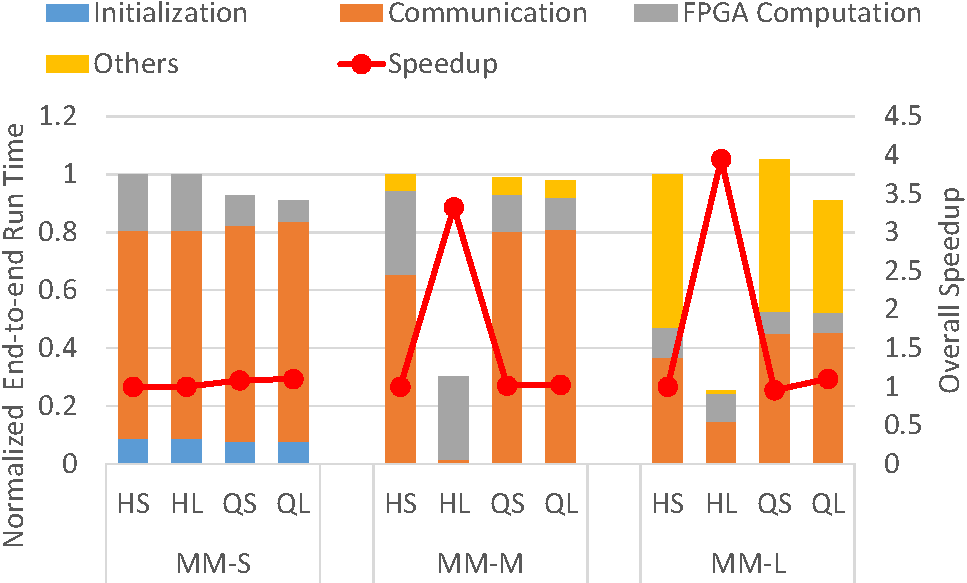
\includegraphics[width=0.46\linewidth]{mm-real-perf}}
\qquad
\subfloat[FIR]{
\label{fig:fir-real-perf}
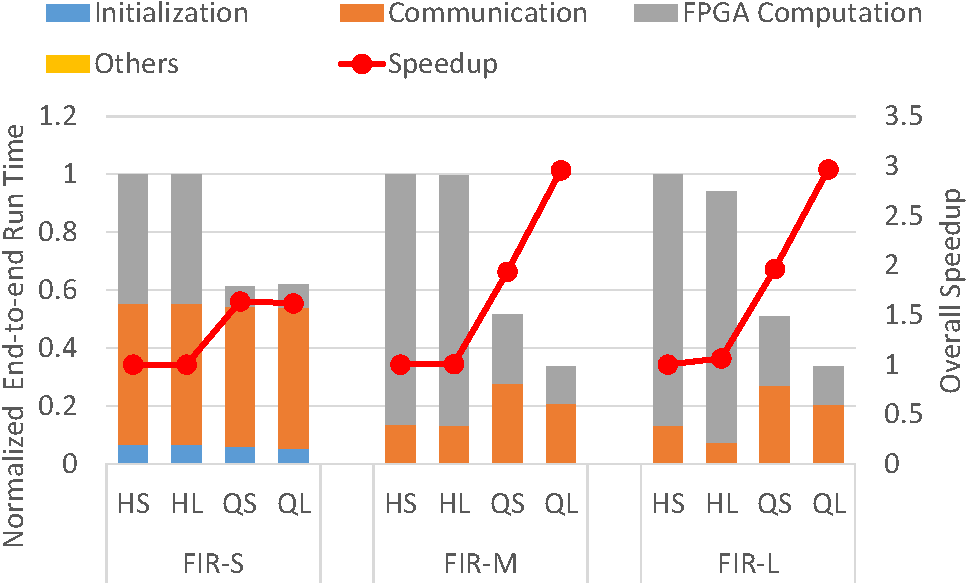
\includegraphics[width=0.46\linewidth]{fir-real-perf}}
\qquad
\subfloat[SE]{
\label{fig:sobel-real-perf}
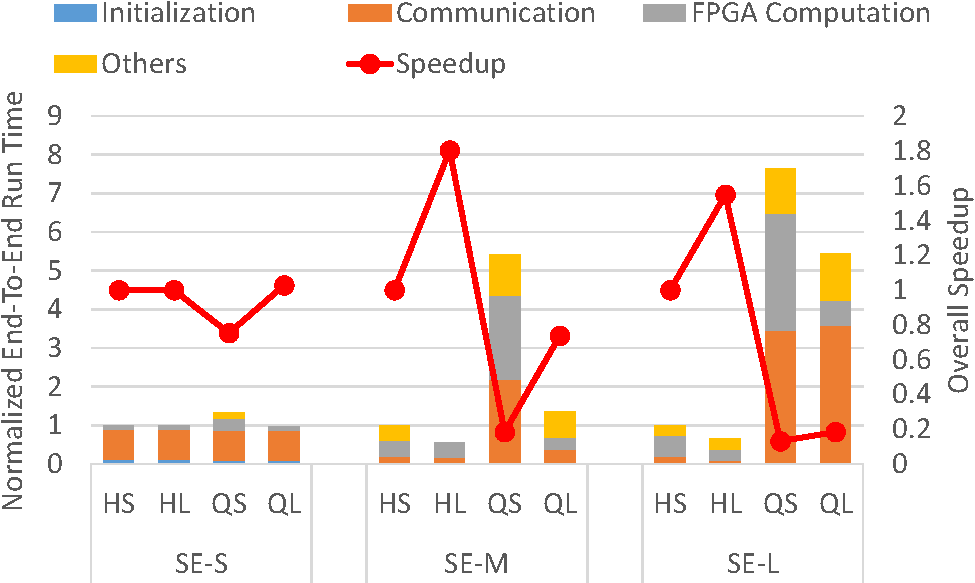
\includegraphics[width=0.46\linewidth]{sobel-real-perf}}
\qquad
\subfloat[KM]{
\label{fig:kmean-real-perf}
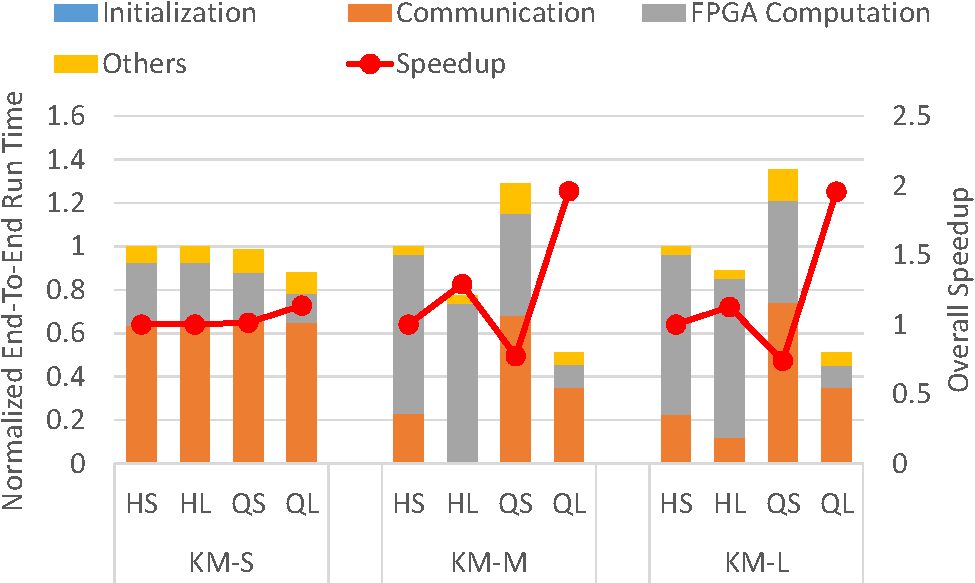
\includegraphics[width=0.46\linewidth]{kmean-real-perf}}
\caption{Benchmark Speedup and Execution Time Decomposition Using Both Direct HLS Based Design
Framework and QuickDough. HS is used as the baseline design to calculate the speedup as well as the
normalized execution time.}
\label{fig:real-perf}
\end{figure}

The results in the figure illustrate the complex relationship between accelerator configurations and
the structure of the application on performance. Typically, performance of the accelerators
generated using QuickDough is in the same order of those created using a direct HLS-based
methodology.  In the extreme cases, such as FIR-M and FIR-L, the QuickDough accelerator's
performance is $3\times$ better, while in other cases, such as SE-M and SE-L, they can be up
to $7.3\times$ slower. The variation in performance is due to the intricate interaction between the
accelerator architecture, the computation and data reuse pattern of the user application.

To further investigate the computing performance of the accelerators, \figref{fig:kernel-sim-perf}
further breaks down the results, showing only the simulated computing time spent in the
accelerators. The performance impacts due to communication, data organization, as well as
implementation frequency are not shown.

\begin{figure}
\center{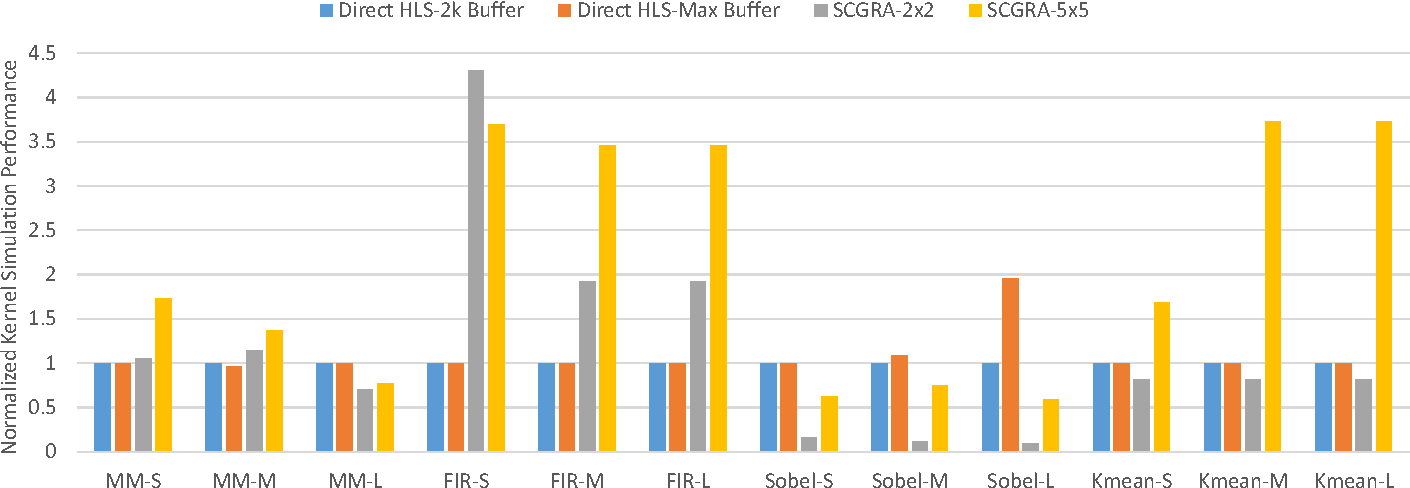
\includegraphics[width=0.8\linewidth]{kernel-sim-perf}}
\caption{Compute Kernel Simulated Performance Using Both Direct HLS Based Design Framework and
QuickDough. The performance is normalized to that of HS.}
\label{fig:kernel-sim-perf}
\end{figure}

In the case of MM, the QuickDough generated accelerators performed similar to HS with all matrix
sizes. In these 3 cases, the QuickDough accelerators exhibit slightly higher communication cost,
which is compensated by their slightly shorter time spent in computation. In fact, the QuickDough
accelerators perform slightly better in both MM-S and MM-M as can be seen in
\figref{fig:kernel-sim-perf}. However, HL outperform all cases by up to a factor of 4. It is
because its large input buffer is able to buffer all input data on-chip, essentially eliminating the
communication cost between the CPU and FPGA. The QuickDough overlay cannot afford buffer of this
size as on-chip memories are devoted to the overlay execution.

In the case of FIR, we see that the QuickDough accelerators outperform the rest regardless of the
input data size.  In these cases, the communication cost is comparable while the QuickDough
accelerators have a clear advantage in computing time as shown in \figref{fig:kernel-sim-perf}. Part
of the reason is that the FIR application can be unrolled at least \num{20} times more in the
QuickDough accelerators than the HLS-based accelerators, shown in
\tabref{tab:loop-unrolling-setup-vivado} and \tabref{tab:loop-unrolling-setup-scgra}. The heavily
unrolled loops provide far more operations to be carried out in parallel that lead to lower
computing time. On the other hand, unrolling is limited in HLS tools due to the limited available
resources. The commercial HLS tools were not very effective in time-sharing the generated blocks.

In the case of KM, similar observation can be made in terms of loop unrolling. As shown in
\figref{fig:kernel-sim-perf}, the larger processing array in QL is able to take advantage of the
heavily unrolled loops, while the smaller array size in QS limits the achievable speedup. However,
because of the higher communication cost, the overall speedup is limited.

Finally, in the case of SE, the QuickDough generated accelerators perform poorly compared to those
generated using HLS tools. Comparing \figref{fig:real-perf} and \figref{fig:kernel-sim-perf}, we can
see that the QuickDough accelerators not only spend more time in communication, but they are also
slower in computing. In terms of computation, we see that the high-level synthesis tools are capable
of simplify the user-provided computation effectively through constant propagation. On the other
hand, the constant multiplications must be carried out regardless in the QuickDough overlay,
generating a lot more operations comparatively. At the same time, the large number of additional
compute operations in the QuickDough accelerators significantly increases the compute-to-I/O ratio
of the accelerators. As a result, only small portion of input data can be transferred in groups
before a new batch of data must be transferred. This increased number of transfer between FPGA and
CPU significantly limits the overall system performance.

\subsubsection{Implementation Frequency}
One advantage of employing a simple and regular overlay architecture is that it allows for highly
optimized physical implementations. In particular, when compared to the random hardware generated by
HLS tools, the QuickDough overlay is regular and highly pipelined, allowing implementations to run
at much higher frequencies.  The increased running frequency in turns results in higher overall
performance of the system.


\begin{figure}
\center{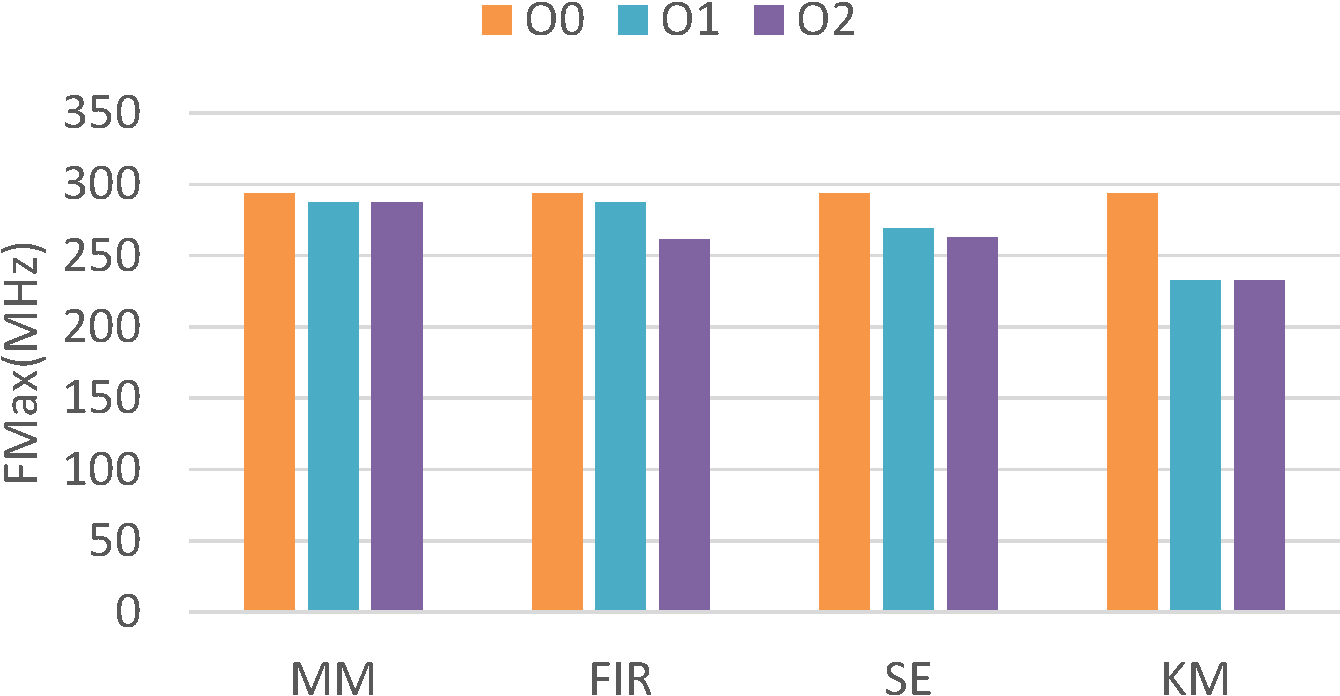
\includegraphics[width=0.8\linewidth]{impl-freq}}
\caption{Implementation Frequency of The Accelerators Using Both Direct HLS Based Design Framework and QuickDough}
\label{fig:impl-freq}
\end{figure}

\figref{fig:impl-freq} shows the implementation frequency of the benchmark using both design
methodologies. Direct HLS based design framework takes timing constrain into consideration at the
HLS step, and it can either synthesize the compute kernel to a lower frequency design with better
simulated performance or a higher frequency design with worse simulation performance. Neither of
them have a clear advantage over the other.  In these experiments, the implementation tools were
targeting a \SI{100}{\mega\hertz} clock that the AXI controller on the Zedboard typically works at.
Even at this rate, some of the synthesized IP cores could barely meet timing.

On the other hand, QuickDough utilizes the SCGRA overlay as the hardware infrastructure. Since the
SCGRA overlay is regular and pipelined, the implementation frequency of the accelerator built on top
of the SCGRA overlay is much higher than that of the accelerator produced using direct HLS. QS with
a $2\times 2$ SCGRA overlay can run at \SI{200}{\mega\hertz} while QL with a $5 \times 5$ SCGRA
overlay can run at \SI{167}{\mega\hertz}. The implementation frequency degrades slightly
with a large design because more than \SI{90}{\percent} of the BRAM blocks on target FPGA are used
and the routing becomes extremely tight. 

\subsection{Compilation Time} \label{subsec:compilation}
In this section, the compilation time of the QuickDough framework is compared against that of using a direct HLS synthesis methodology.  It is used as an indicator on the designer's productivity as it greatly limits the number of debug-edit-implementation cycles achievable per day.

\subsubsection{Direct HLS-based design}
The baseline direct HLS-based design framework consists of 4 main steps:
 
\begin{itemize}[label=\textbullet,leftmargin=2em,rightmargin=\leftmargin]
%\renewcommand\labelitemi{$\bullet$}
%\setlength\itemindent{1em}
\item Compute kernel synthesis: The compute kernel is translated to the corresponding HDL model.
\item Kernel IP generation: The compute kernel is synthesized and packed as an IP core.
\item Accelerator implementation: The FPGA accelerator built on top of the IP core is implemented. 
\item Software compilation: The application employing the FPGA accelerator is compiled to binary code.
\end{itemize}

The time to generate our benchmark accelerators through these steps is shown in \figref{fig:Vivado-HLS-Compilation-Time}.
From the figure, it is clear that IP core generation and hardware implementation dominate the compilation time, taking upward of almost an hour to implement some benchmark applications.
Comparatively, the time for software compilation and kernel synthesis are negligible in most cases.
Unfortunately, under this design methodology, every implementation iteration must go through all 4 steps, even when only minor modifications were needed.
This long debug-edit-implement cycle greatly limits the designer's productivity.

\begin{figure}
\center{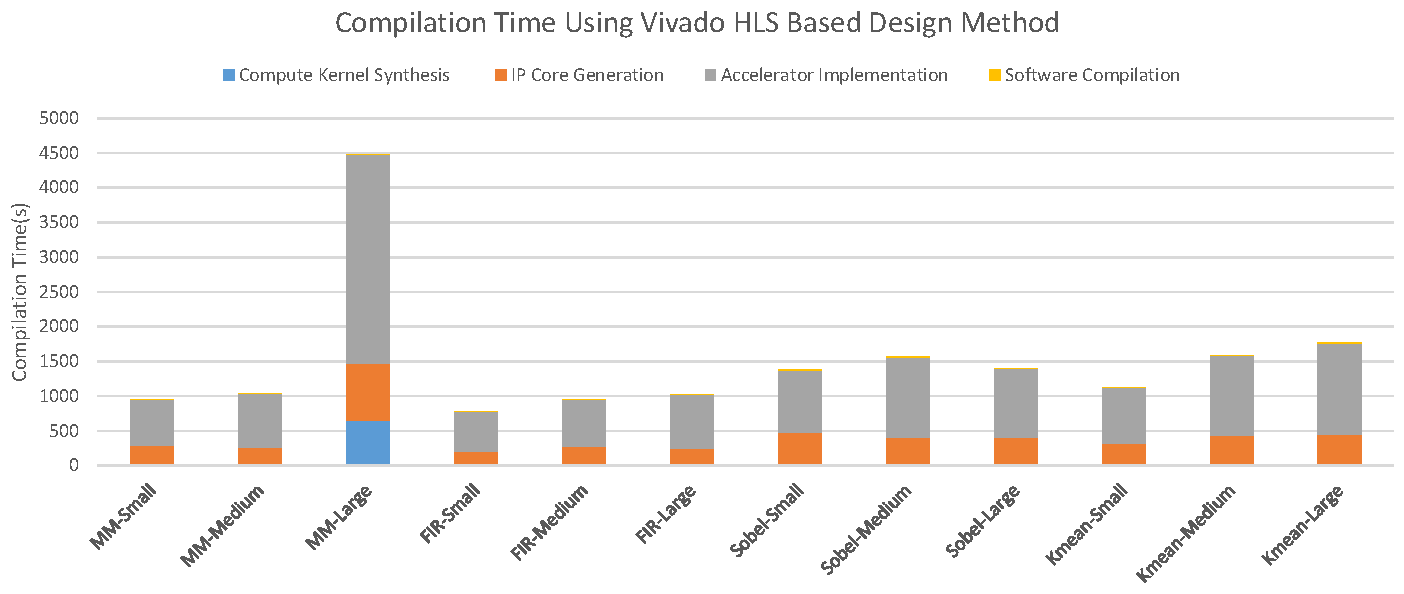
\includegraphics[width=0.8\linewidth]{HLS-Compilation-Time}}
\caption{Benchmark Compilation Time Using Direct HLS Based Design Framework}
\label{fig:Vivado-HLS-Compilation-Time}
\end{figure}

\subsubsection{QuickDough Compilation Time}
Every implementation iterations in QuickDough also involves 4 steps:

\begin{itemize}[label=\textbullet,leftmargin=2em,rightmargin=\leftmargin]
%\renewcommand\labelitemi{$\bullet$}
%\setlength\itemindent{1em}
\item DFG generation: The compute kernel is translated to corresponding DFG.
\item DFG scheduling: The DFG is scheduled to the customized SCGRA overlay. 
\item Bitstream generation: The scheduling result is embedded into a pre-built accelerator bitstream 
to produce the final FPGA bitstream of the compute kernel.
\item Software compilation: Application using the SCGRA accelerator is compiled to binary code.
\end{itemize}



\figref{fig:SCGRA-Overlay-Compilation-Time} shows the compilation time of our benchmark using QuickDough.
Except for DFG scheduling, all remaining steps are fast and consume about constant time across different applications.
DFG scheduling is relatively slower and its run time depends on the DFG and SCGRA overlay size.
Yet, this longest step does not last longer than a few seconds for all our benchmarks.
Overall, QuickDough is able to reimplement an application in 5 to 15 seconds, a two orders of magnitude improvement over our baseline direct HLS-based design framework.

\begin{figure}
\center{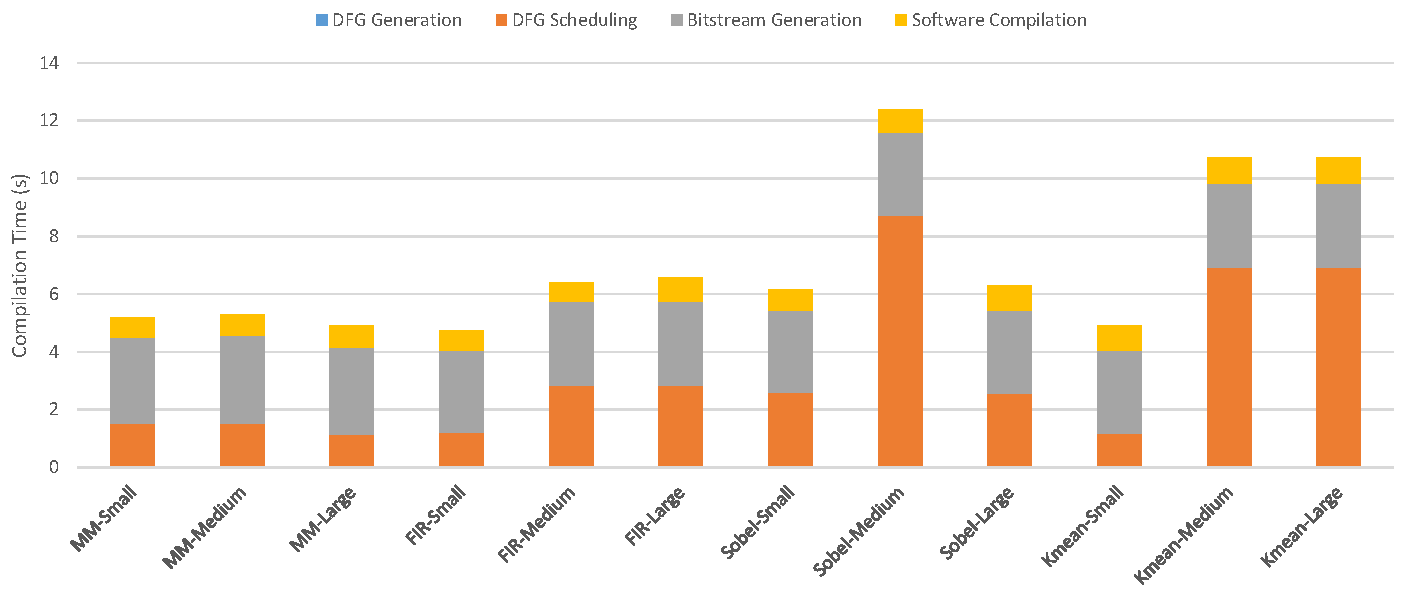
\includegraphics[width=0.8\linewidth]{QuickDough-Compilation-Time}}
\caption{Benchmark Compilation Time Using QuickDough}
\label{fig:SCGRA-Overlay-Compilation-Time}
\end{figure}


Clearly, the designer must spend the time to physically implement the overlay architecture on the target FPGA, spending considerable time on the implementation tools.
However, this can be done only as needed, for example, on a per-application-domain basis.
The designer may iterate via the above rapid steps during design and debugging phases using a initial overlay implementation.
Once the functionality is frozen, the designer may then opt to further optimize performance through overlay customization and reimplement a different overlay architecture.
We argue that the ability to separate functionality and optimization concern, and the possibility of performing rapid debug-edit-implement iterations in QuickDough are crucial factors that contribute to a high-productivity design experience.



%On top of the compilation time, the abstraction level of the design entry, design reuse and portability are also important aspects that affect the design productivity. Both direct HLS based design framework and QuickDough adopt sequential high level language C/C++ as design input, but QuickDough still needs further efforts to have the DFG generation done automatically. Direct HLS based design framework needs the compute kernel be synthesized and implemented for each application instance. QuickDough requires compilation for each application instance as well, but it can reuse the same hardware infrastructure across the applications in the same domain. It is possible for direct HLS based design framework to port the synthesized HDL design among different devices and parts, but IP core generation and accelerator implementation depend on specific FPGA device and they are needed for each application instance. QuickDough's portability is also limited at HDL level, and complete hardware implementation is needed to port to a different FPGA device.

\subsection{Implementation Overhead} \label{subsec:impl}
In this section, hardware implementation overhead in both design methodologies are compared. Furthermore, we examined the impact on overlay customization on implementation overhead.

\subsubsection{General Overlay Architecture}
\tabref{tab:hardware-overhead-comparison} shows the hardware overhead of both accelerator design methodologies across the benchmark applications.
In these cases, an identical and general overlay architecture was employed across all benchmark applications.

\begin{table}
\footnotesize 
\centering
\tbl{Hardware Overhead of The Accelerators Using Both Direct HLS Bsed Design Framework and QuickDough \label{tab:hardware-overhead-comparison}}{
  \resizebox{0.55\columnwidth}{!}{
\begin{tabular}{l|l|l|l|l|l|l}
\hline
\multicolumn{3}{l|}{} & FF  & LUT & RAM36 & DSP48 \\ \hline 
\multirow{6}{*}{MM} & \multirow{3}{*}{ \tabincell{c}{HS}} & S & 4812 & 3390 & 4 & 84 \\ \cline{3-7} 
                    &                            & M & 4804 & 4703 & 4 & 12 \\ \cline{3-7} 
                    &                            & L & 11107 & 11524 & 4 & 12 \\ \cline{2-7}
                    & \multirow{3}{*}{ \tabincell{c}{HL}} & S & 4826 & 3390 & 128 & 84 \\ \cline{3-7} 
                    &                             & M &  4251 & 4866 & 128 & 9 \\ \cline{3-7} 
                    &                             & L & 11024 & 24890 & 128 & 12 \\ \hline

\multirow{6}{*}{FIR} & \multirow{3}{*}{ \tabincell{c}{HS}} & S & 3736 & 3570 & 4 & 27 \\ \cline{3-7} 
                     &                            & M & 3756 & 3872 & 4 & 27  \\ \cline{3-7} 
                     &                            & L & 3756 & 3872 & 4 & 27 \\ \cline{2-7}
                     & \multirow{3}{*}{ \tabincell{c}{HL}} & S & 3742  & 3570 &  128 & 27 \\ \cline{3-7} 
                     &                             & M & 3782 & 4246 & 128 & 27 \\ \cline{3-7} 
                     &                             & L & 3792 & 4426 & 128 & 27 \\ \hline

\multirow{6}{*}{SE} & \multirow{3}{*}{ \tabincell{c}{HS}} & S & 9556 & 6467 & 6 & 216 \\ \cline{3-7} 
                       &                            & M & 7483 & 5520 & 6 & 144 \\ \cline{3-7} 
                       &                            & L & 7102 & 5501 & 6 & 144 \\ \cline{2-7}
                       & \multirow{3}{*}{ \tabincell{c}{HL}} & S & 9564 & 6467 & 130 & 216 \\ \cline{3-7} 
                       &                             & M & 7496 & 5711 & 130 & 144 \\ \cline{3-7} 
                       &                             & L & 7622 & 5904 & 130 & 144 \\ \hline

\multirow{6}{*}{KM} & \multirow{3}{*}{ \tabincell{c}{HS}} & S & 2826 & 3567 & 4 & 24 \\ \cline{3-7} 
                       &                            & M & 6709 & 8088  & 4 & 120 \\ \cline{3-7} 
                       &                            & L & 6709  & 8088  & 4  & 120 \\ \cline{2-7}
                       & \multirow{3}{*}{ \tabincell{c}{HL}} & S & 2852 & 3567 & 128 & 24 \\ \cline{3-7} 
                       &                             & M & 6754 & 8122 & 128 & 120 \\ \cline{3-7} 
                       &                             & L & 6770 & 8205 & 128 & 120 \\ \hline

\multicolumn{3}{l|}{QS} & 9302 & 5745 & 32 & 12  \\ \hline
\multicolumn{3}{l|}{QL} & 34922 & 21436 & 137 & 75 \\ \hline
\multicolumn{3}{l|}{Total FPGA Resource} & 106400 & 53200 & 140 & 110 \\ \hline
\end{tabular}
}
}
\end{table}

From the table, it is clear that the accelerators using direct HLS based design framework generally consume fewer flip-flops, LUTs and RAM36s due to the delicate customization for each application instance. However, the number of DSP48 required increases significantly with the expansion of the application kernel and it limits the maximum loop unrolling factors for many applications. 

On the other hand, the accelerators using QuickDough usually require comparable number of DSP48s, more FFs, LUTs and RAM36s.  In particular, the large consumption of RAM36s often becomes the bottleneck limiting the maximum SCGRA size that can be implemented on the target FPGA.
This limited size in turn constrains the maximum loop unrolling and blocking of the application and thus the overall performance.

\subsubsection{Overlay Customization}
To investigate the effect of overlay customization on hardware overhead, we further divided the four
benchmarks into three groups.  In the first group, since MM and FIR share the same set of compute
operations, they were implemented using the same customized overlay.  In the second case, since SE
does not require a complete \num{32}-bit data path, a customized overlay with a mixed of
\num{16}-bit and \num{32}-bit data path was used.  Finally, since KM requires almost all the operations presented in the original overlay, no change was made.

The experiments were rerun using the respective customized overlay and the resulting hardware savings are shown in \figref{fig:hardware-saving}.  Overall, the customized overlays provide as much as \SI{65}{\percent} of DSP48, \SI{30}{\percent} of LUT, as well as \SI{15}{\percent} of FFs saving over the original generic design.

\begin{figure}
\center{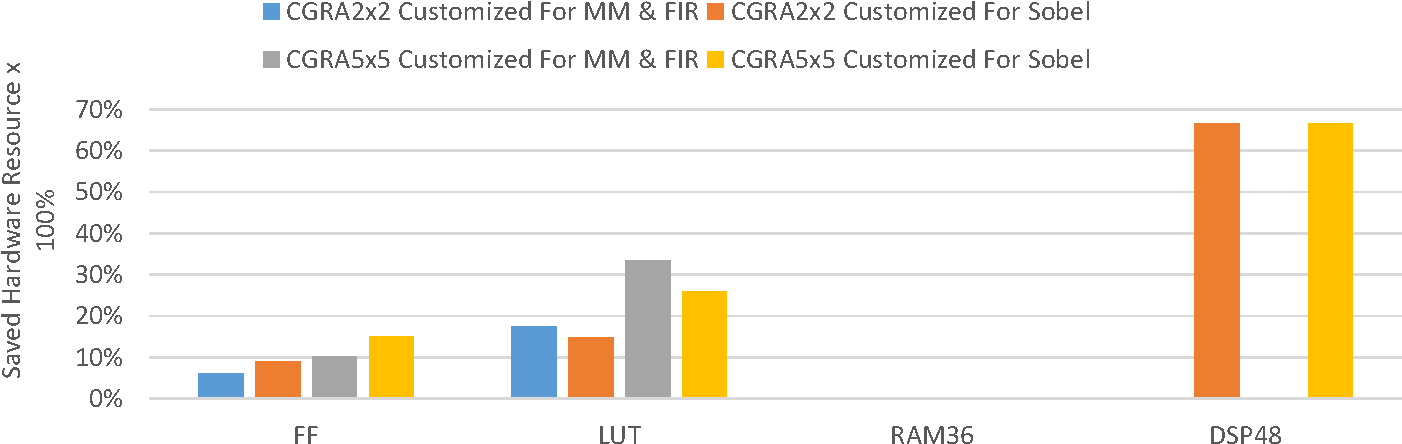
\includegraphics[width=0.7\linewidth]{hardware-saving}}
\caption{Hardware Saving Of Customized SCGRA Overlay}
\label{fig:hardware-saving}
\end{figure}


  
\subsection{Scalability} \label{subsec:scalability}
Finally, we studied the scalability of the proposed overlay architecture in terms of problem size as
well as processing array size in anticipation for future FPGA devices.

\subsubsection{Problem Size}
To study the effect of problem size on the overlay performance, MM with
matrix sizes ranging from $4\times 4$ to $20 \times 20$ were used. In the case of QuickDough
overlay, \num{3} different SCGRA sizes were studied: $2\times 2$, $5\times 5$, $10\times 10$. They
were targeted at the larger \texttt{zc706} FPGA with abundant hardware resource. In the case of
direct HLS synthesis, \num{2} scenarios were considered.  In the first scenario, the matrix
multiplication was fully unrolled. In the second scenario, a best-effort loop unrolling that results in
maximum performance under hardware constraints was used. In the case of the SCGRA overlay, the
MM operations were fully unrolled. \figref{fig:mm-sim-perf} shows the simulated
performance of the resulting accelerators generated by both design methodologies. Communication
cost was not taken into account as they remain comparable in both cases.

\begin{figure}
\centering
\subfloat[]{
\label{fig:mm-sim-perf1}
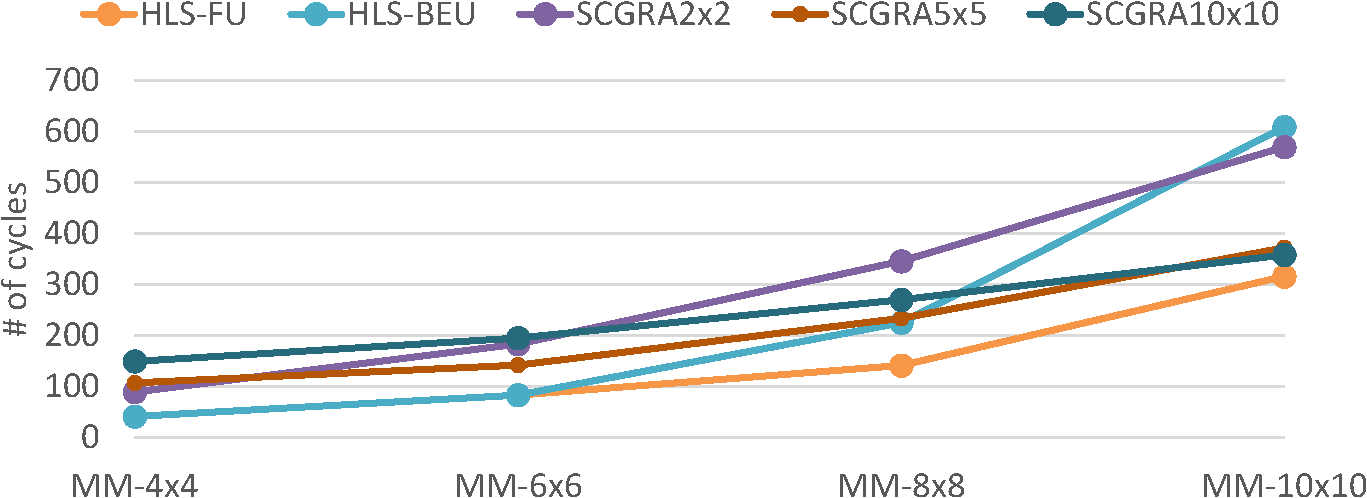
\includegraphics[width=0.45\linewidth]{mm-sim-perf1}}
\qquad
\subfloat[]{
\label{fig:mm-sim-perf2}
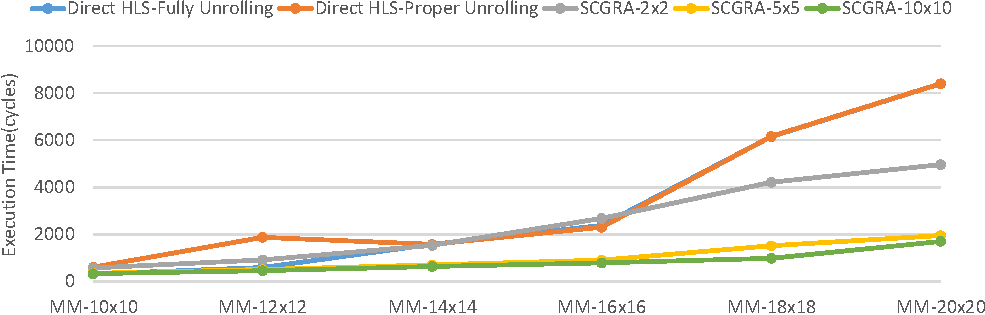
\includegraphics[width=0.45\linewidth]{mm-sim-perf2}}
\caption{Simulated Performance Of MM Implemented Using Both Direct HLS Based Design Framework And QuickDough}
\label{fig:mm-sim-perf}
\end{figure}

Results from the figure show that accelerators using direct HLS based design framework perform much
better than the QuickDough accelerators when the matrix size is small enough for the loops to be
fully unrolled. However, as the matrix size grows, direct HLS can no longer afford the hardware overhead for
intensive loop unrolling, limiting the performance of the resulting accelerators. As shown in
\figref{fig:loop-unroll-and-pipeline}, the DSP resource consumption increases significantly with
additional unrolling in return for higher performance as the matrix size increases.  While it is
possible for an expert to start manually time-sharing the resources, we did not explore such
sophisticated implementation technique in attempt to maintain a comparable design effort.

\begin{figure}
\center{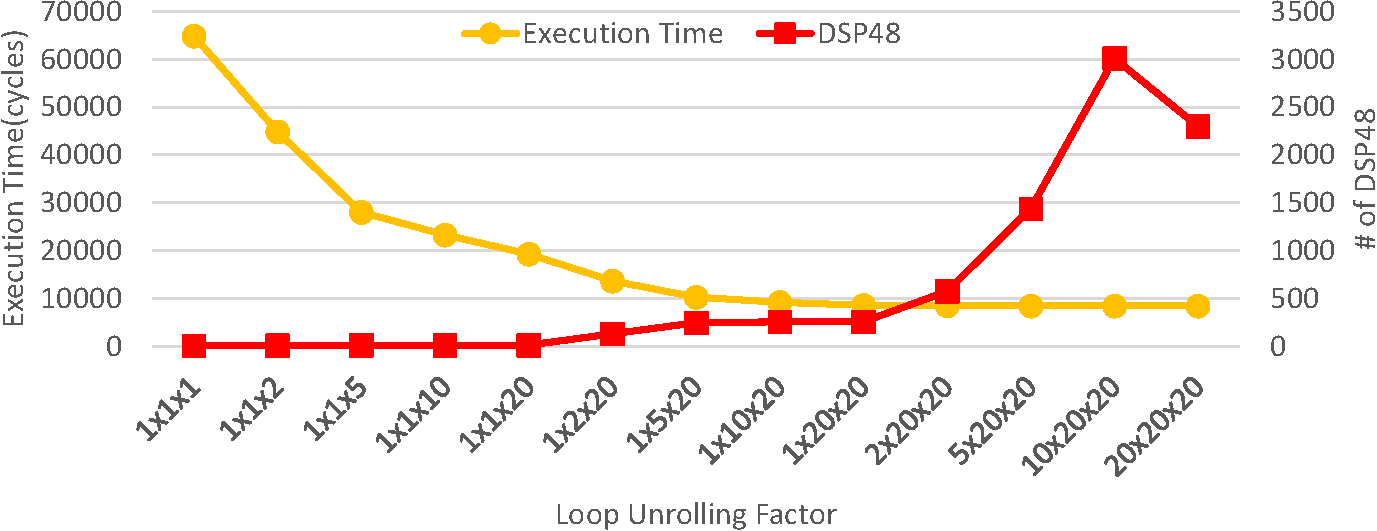
\includegraphics[width=0.7\linewidth]{hls-loop-unroll}}
\caption{MM 20x20 Implemented Using Direct HLS Based Design Framework With Diverse Loop Unrolling}
\label{fig:loop-unroll-and-pipeline}
\end{figure}

On the other hand, the QuickDough overlay can naturally accommodate intensive loop unrolling through
time-sharing of hardware resources. It is therefore capable of accelerating much larger portion of
computation with relative ease. Its performance is mainly limited by the on-chip memory serving as
instruction ROMs.

In our experiments with MM that target the larger \texttt{zc706} device, MM-8x8 is the crossover point that QuickDough begins to outperform.  As a comparison, the crossover point on the originally targeted Zedboard was much smaller because of the limited hardware resource.




\subsubsection{Overlay Processing Array Size}
To study the scalability of our SCGRA overlay, the performance of processing array with increasing size was experimented using MM-20x20 as an example.

\figref{fig:scalability-performance} shows that in general, the additional processing power provided by the larger arrays results in better performance as expected.
The performance gain reduces as the array size increases to a point when there simply is not enough available compute operations to be scheduled.
This point of reflection depends on the nature of the user application.
In the case of MM, the $5 \times 5$ array provided the near-optimal performance with reasonable amount of PEs.

\begin{figure}
\centering
\subfloat[Performance]{\label{fig:scalability-performance}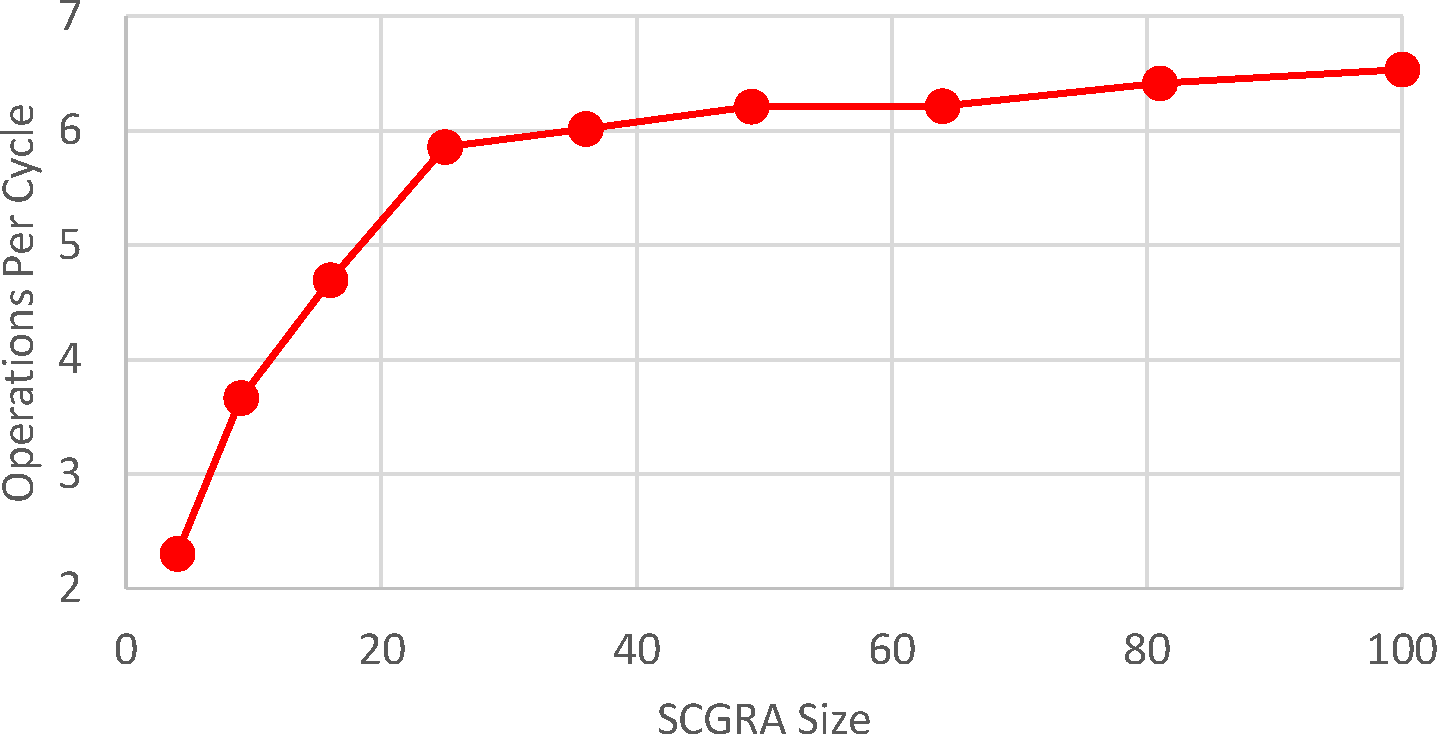
\includegraphics[width=0.45\linewidth]{perf-scale}}
\hfill
\subfloat[Overhead \& frequency]{\label{fig:scgra-overhead-scalability}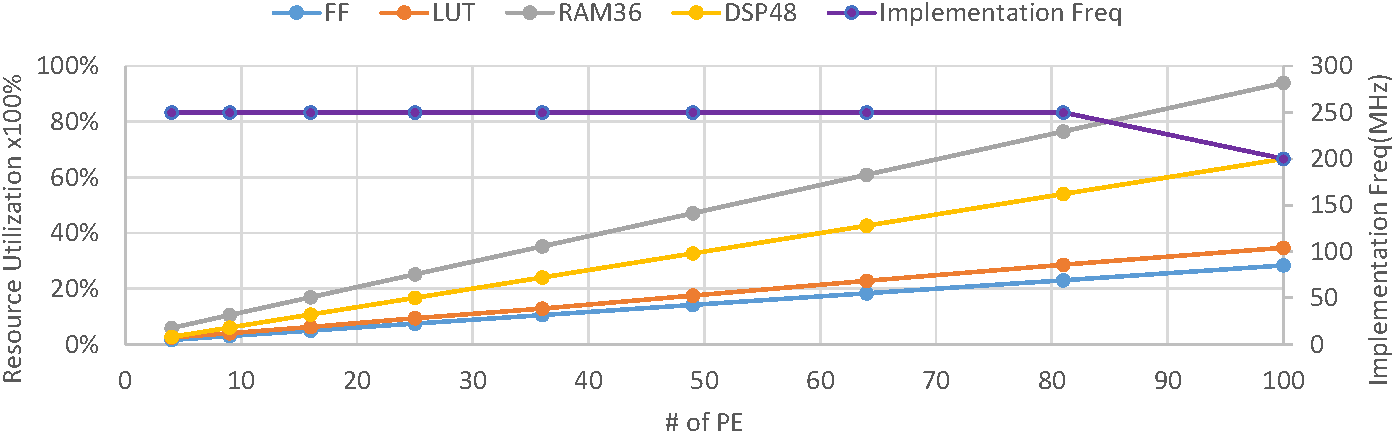
\includegraphics[width=0.45\linewidth]{scgra-impl-scalability}}
\caption{Simulated performance, hardware overhead and implementation frequency of MM-20 implemented with increasing SCGRA overlay size.}

\end{figure}


As an overlay design, it is important that its design should allow flexible scaling of its computing power to address the needs from the application.
As a simple, fully synchronous and highly regular reconfigurable array, the QuickDough overlay is very much scalable in that dimension as shown in 
\figref{fig:scgra-overhead-scalability}.

From the figure, it can be seen that the hardware overhead associated with the QuickDough overlay increases linearly with the number of processing elements in the array.  Most importantly, except for the largest array when the FPGA is almost full, it the QuickDough overlay is able to run at a constant high clock frequency.

%Finally, we also compare the implementation frequency using both design methodologies. Since the maximum clock available is 250MHz and the speed level of FPGA on Zc706 is -2, the implementation using both design methodologies present similar implementation frequency. QuickDough allows SCGRA ranging from 2x2 to 9x9 running at 250MHz on Zc706. SCGRA 10x10 degrades slightly and can still work at 200MHz. Direct HLS has all the implementation running at 200MHz. 


